\documentclass[fleqn]{hw}

\usepackage{url}
\usepackage{graphicx}
\usepackage{amsmath}
\title{HW4: Reinforcement Learning}
\duedate{}
\class{CS6300: Artificial Intelligence}
\institute{University of Utah}
\author{Jake Pitkin}
% IF YOU'RE USING THIS .TEX FILE AS A TEMPLATE, PLEASE REPLACE
% The author WITH YOUR NAME AND UID.
% Replace the due date with anyone you worked with i.e. "Worked with: John McCarthy, Watson, & Hal-9000"
\begin{document}
\maketitle

% IF YOU'RE USING THIS .TEX FILE AS A TEMPLATE, PLEASE REPLACE
% "CS5300, Spring 2009" WITH YOUR NAME AND UID.

% Hand in at: http://www.cs.utah.edu/~hal/handin.pl?course=cs5300

\section{TD and Q in Blockworld}

Consider the following gridworld:
\begin{figure}[h!]
  \centering
  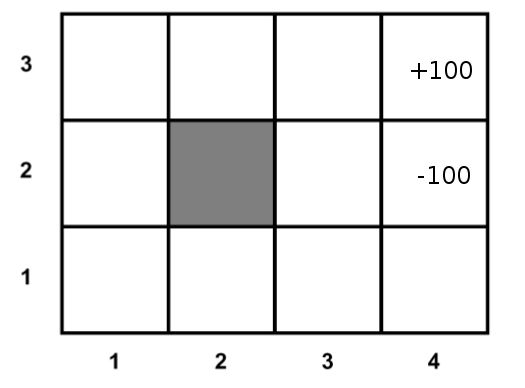
\includegraphics[width=0.6\textwidth]{GridWorld}
\end{figure}

Suppose that we run two episodes that yield the
following sequences of (state, action, reward) tuples:

\begin{tabular}{ccc|ccc}
{\bf S} & {\bf A} & {\bf R} & {\bf S} & {\bf A} & {\bf R} \\
\hline
(1,1) & up    & -1     & (1,1) & up    & -1 \\
(2,1) & left  & -1     & (1,2) & up    & -1 \\
(1,1) & up    & -1     & (1,3) & right & -1 \\
(1,2) & up    & -1     & (2,3) & right & -1 \\
(1,3) & up    & -1     & (2,3) & right & -1 \\
(2,3) & right & -1     & (3,3) & right & -1 \\
(3,3) & right & -1     & (4,3) & exit  & +100 \\
(4,3) & exit  & +100   & (done)&       & \\
(done)&       &        &       &       & \\
\end{tabular}

\begin{enumerate}
    \item {\bf According to direct estimation, what are the values for every state in the grid?}

\begin{center}
\begin{tabular}{c|c|c}
    {\bf State} & {\bf Calculation} & {\bf Value} \\
\hline
    (1,1) & (93 + 95 + 94)/3 & 94 \\
    (1,2) & (96 + 95)/2&95.5 \\
    (1,3) & (97 + 96)/2&96.5 \\
    (2,1) & 94/1&94 \\
    (2,2) & -&- \\
    (2,3) & (98 + 97 + 98)/3&97.666 \\
    (3,1) & -&- \\
    (3,2) & -&- \\
    (3,3) & (99 + 99)/2&99 \\
    (4,1) & -&- \\
    (4,2) & -&- \\
    (4,3) & (100 + 100)/2&100 \\
\end{tabular}
\end{center}

    \item {\bf According to model-based learning, what are the transition
probabilities for every (state, action, state) triple.  Don't bother
        listing all the ones that we have no information about. }

\begin{center}
\begin{tabular}{c|c|c|c}
{\bf s} & {\bf a} & {\bf s$^\prime$} & {\bf T(s, a, s$^\prime$)} \\
\hline
(1,1) & up & (2,1) & 1/3\\
(1,1) & up & (1,2) & 2/3\\
(1,2) & up & (1,3) & 1\\
(1,3) & up & (2,3) & 1\\
(1,3) & right & (2,3) & 1\\
(2,1) & left & (1,1) & 1\\
(2,3) & right & (3,3) & 2/3\\
(2,3) & right & (2,3) & 1/3\\
(3,3) & right & (4,3) & 1\\
(4,3) & exit & (done) & 1\\
\end{tabular}
\end{center}

\item {\bf Suppose that we run Q-learning.  However, instead of initializing all
our Q values to zero, we initialize them to some large positive number
(``large'' with respect to the maximum reward possible in the world:
say, 10 times the max reward).  I claim that this will cause a
Q-learning agent to initially explore a lot and then eventually start
exploiting.  Why should this be true?  Justify your answer in a short
        paragraph.}
\end{enumerate}

\section{Policy Gradient}

In order to do policy gradient, we need to be able
to compute the gradient of the value function $J$ with respect
to a parameter vector ${\mathbf \theta}$: $\nabla_{\mathbf \theta} J(\theta)$.  By
our algebraic magic, we expressed this as:

\begin{equation} \label{eq:grad}
\nabla_{\mathbf \theta} J(\mathbf \theta) 
  = \sum_a \pi_{\mathbf \theta}(s_0,a) R(a) 
             \underbrace{\nabla_{\mathbf \theta} \log \left( \pi_{\mathbf \theta}(s_0,a) \right)}_{g(s_0,a)}
\end{equation}

If we us a linear function thrown through a soft-max as our stochastic
policy, we have:

\begin{equation}
\pi_{\mathbf \theta}(s,a) 
  = \frac {\exp \left( \sum_{i=1}^n \theta_i f_i(s,a) \right)}
          {\sum_{a'} \exp \left( \sum_{i=1}^n \theta_i f_i(s,a') \right)}
\end{equation}

{\bf Compute a closed form solution for $g(s_0,a)$.} 

We are given that:

$$g(s_0, a) = \nabla_\theta = log\bigg[\frac {\exp \left( \sum_{i=1}^n \theta_i f_i(s,a) \right)}
          {\sum_{a'} \exp \left( \sum_{i=1}^n \theta_i f_i(s,a') \right)}
\bigg]$$


{\bf Explain in a few
sentences \emph{why} this leads to a sensible update for gradience
ascent (i.e., if we plug this in to Eq~\eqref{eq:grad} and do gradient
ascent, why is the derived form reasonable)?}

\end{document}

%%% Local Variables:
%%% mode: latex
%%% TeX-master: t
%%% End:
